\section{Theorie}
\label{sec:Theorie}
\subsection{Aufbau einer Kathodenstrahlröhre}
\begin{figure}
  \centering
  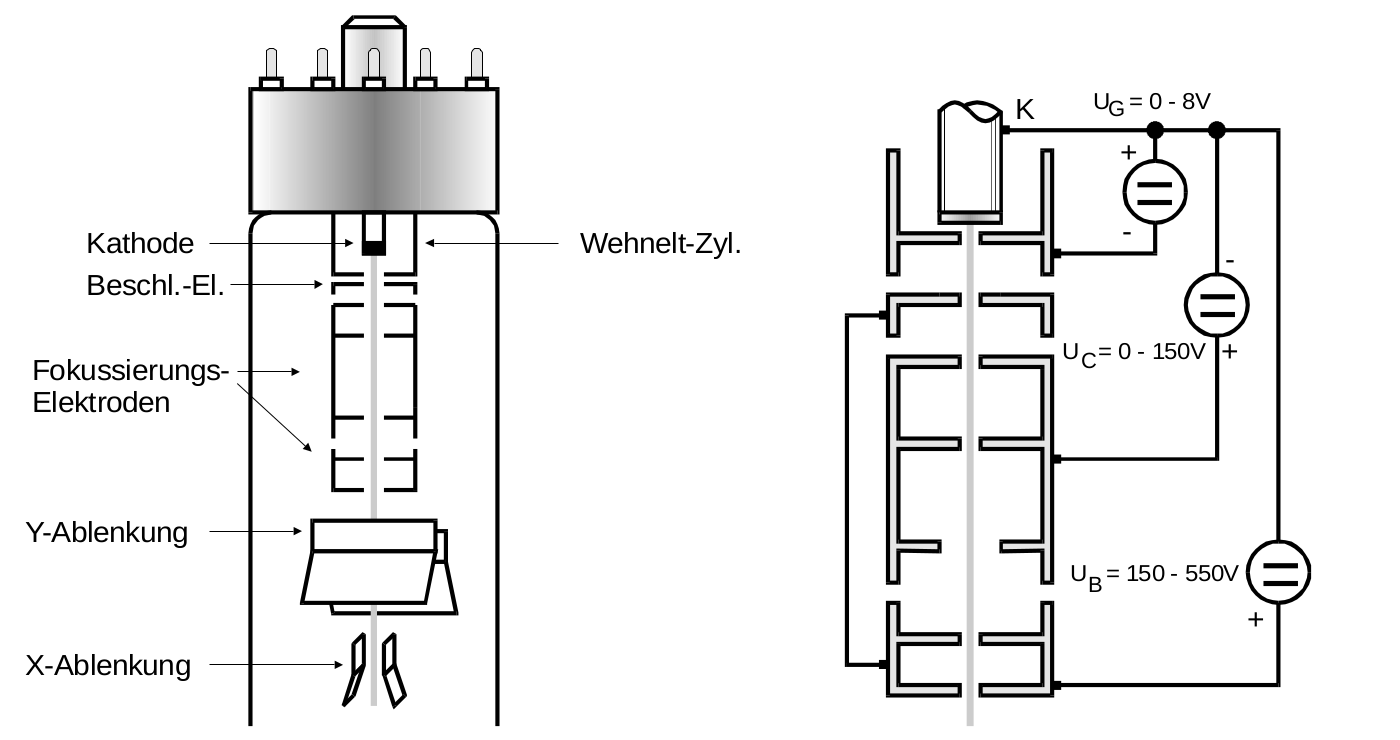
\includegraphics[width=0.8\textwidth]{Messdaten/kathode.png}
  \caption{Prinzipieller Aufbau einer Kathodenstrahlröhre und Schema über die angelegten Potentiale im Fokussierungssystem der Kathodenstrahlröhre.}
  \label{fig:kathode}
\end{figure}
Eine Kathodenstrahlröhre ist ein bis auf einen Restdruck von $\SI{10e-06}{\bar}$ evakuiertes Instrument zur Erzeugung eines möglichst unbeeinflussten Elektronenstrahls.\\
Im Wesentlichen besteht eine Kathodenstrahlröhre aus einer Elektronenkanone, diese erzeugt und fokussiert einen Elektronenstrahl, einem Ablenksystem und einem Leuchtschirm, auf dem der Elektronenstrahl sichtbar gemacht werden kann.\\
Der Elektronenstrahl wird erzeugt an der sogenannten Kathode. Ihre Oberfläche besteht aus einem Material mit niedriger Elektronenaustrittsarbeit.
Die Kathode wird indirekt über eine bis zur Rotglut erhitzten Draht beheizt, sodass
Elektronen aus der Kathode ausgelöst werden.
Umgeben ist die Kathode von dem Wehnelt-Zylinder. Dieser hat ein negatives Potential gegenüber der Kathode, sodass der Elektronenstrahl fokussiert wird. Über das variable Potential des Wehnelt-Zylinders ist es möglich, die Intensität des Elektronenstrahls zu variieren.\\
Vor dem Wehnelt-Zylinder befindet sich, wie in Abbildung \ref{fig:kathode} zu sehen, eine beschleunigende Elektrode. Diese beschleunigt die Elektronen nach dem Energieerhaltungssatz auf
\begin{equation}
  \label{eqn:speedy}
  v_\mathrm{z}=\sqrt{2U_\mathrm{B}\frac{\symup{e}_0}{\symup{m}_0}} \text{.}
\end{equation}
Hinter der beschleunigenden Elektrode befindet sich ein regelbares Fokussierungssystem mit Elektroden verschiedener Potentiale (vgl. dazu \ref{fig:kathode}).
Der Elektronenstrahl wird hierbei über inhomogene elektrische Felder zwischen den Stirnseiten der Fokussierelektroden fokussiert.\\
Der Elektronenstrahl passiert zunächst zwei senkrecht zueinander stehende Plattenpaare, welche bei angelegten Potentialen als Ablenksystem dienen, und trifft schließlich auf den Leuchtschirm. Die auftreffenden Elektronen regen Störstellen im Kristallgitter des Leuchtschirms zur Emission von Photonen an, sodass der Auftreffpunkt des Elektronenstrahls visuell sichtbar wird.
\subsection{Ablenkung eines Elektronenstrahls im elektrischen Feld}
Elektrostatische Felder wirken auf Elektronen. Passiert ein Elektronenstrahl wie in Abbildung \ref{fig:ablenkii} ein annähernd homogenes elektrisches Feld zwischen zwei Ablenkplatten, so wirkt auf jedes Elektron, für die Dauer $\Delta t$ des Aufenthalts im elektrischen Feld, die Kraft
\begin{equation}
  |\vec{F}|=|\symup{e}_0\vec{E}|=\symup{e}_0\frac{U_\mathrm{d}}{d}\text{.}
\end{equation}

Hierbei ist $d$ der Abstand der Ablenkplatten und $U_\mathrm{d}$ das anliegende Potential.\\
Die Durchlaufzeit $\Delta t$ durch das elektrische Feld zwischen den Platten ergibt sich über die Geschwindigkeit der Elektronen in $z$-Richtung mit Gleichung \eqref{eqn:speedy} zu
\begin{equation}
  \Delta t=\frac{p}{v_\mathrm{z}} \text{.}
\end{equation}
Nach dem Passieren der Ablenkplatten hat jedes Elektron eine Geschwindigkeit in $\vec{Y}$-Richtung:
\begin{equation}
  v_\mathrm{y}=F \, \frac{\Delta t}{\symup{m}_0}=\frac{\symup{e}_0}{\symup{m}_0}\frac{U_\mathrm{d}}{d}\cdot\frac{p}{v_\mathrm{z}} \text{.}
\end{equation}
\begin{figure}
  \centering
  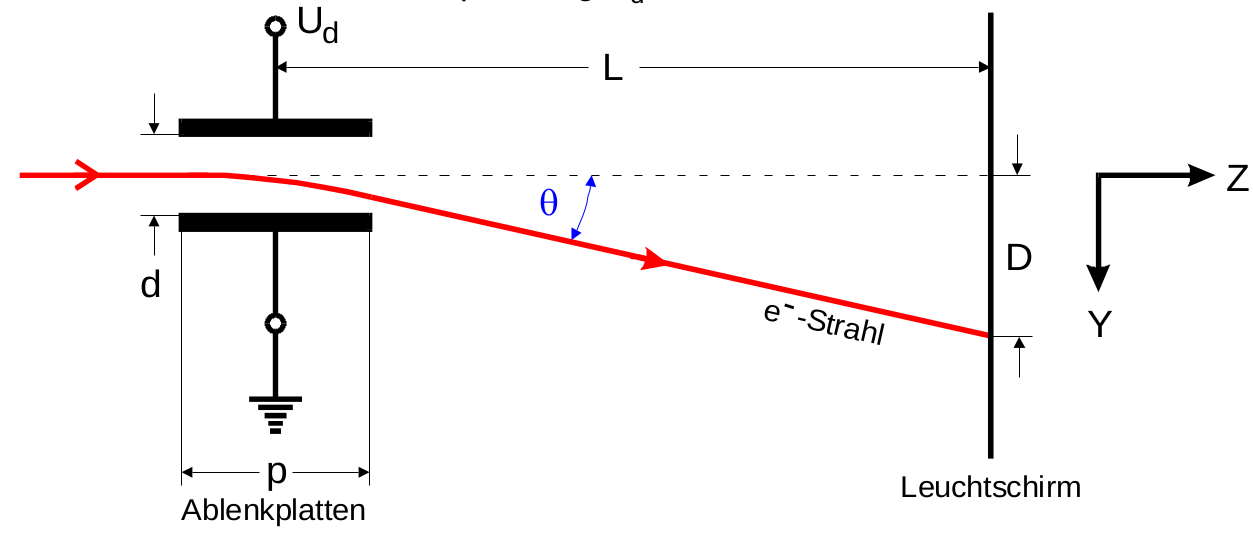
\includegraphics[width=0.98\textwidth]{Messdaten/ablenkung.png}
  \caption{Skizze des Elektronenstrahlverlaufs zur Bestimmung der Verschiebung $D$ des Auftreffpunkts am Leuchtschirm für das elektrische Feld.}
  \label{fig:ablenkii}
\end{figure}
Aus Abbildung \ref{fig:ablenkii} ergibt sich die Verschiebung $D$ des Auftreffpunkts des Elektronenstrahl am Leuchtschirm zu:
\begin{equation}
    D=L \cdot \theta=L \cdot \frac{v_\mathrm{y}}{v_\mathrm{z}}=\frac{\symup{e}_0}{\symup{m}_0}L\frac{U_\mathrm{d}}{d}\frac{p}{v_\mathrm{z}^2} \text{,}
\end{equation}
und unter Verwendung von Gleichung \eqref{eqn:speedy} schließlich
\begin{equation}
  \label{eqn:K}
  D=\frac{p}{2d}L\frac{U_\mathrm{d}}{U_\mathrm{B}} \text{.}
\end{equation}
Es besteht also ein Zusammenhang zwischen der Verschiebung am Leuchtschirm und der Ablenkungspannung. Somit eignet sich die Kathodenstrahlröhre zur Spannungsmessung.
\subsubsection{Der Kathodenstrahl-Oszillograph}
Die Kathodenstrahlröhre kann erweitert werden zu einem Kathodenstrahl-Oszillographen.
Dieser dient zur Untersuchung der Zeitabhängigkeit von Wechselspannungen.\\
Dazu wird auf die Ablenkplatten in $x$-Richtung eine Sägezahnspannung aufgegeben. Eine zweite, über die $y$-Ablenkplatten aufgegebene Spannung kann nun untersucht werden.
\\Stehen die zu untersuchende Wechselspannungsfrequenz $\nu_\mathrm{WS}$ und die Sägezahnspannungsfrequenz $\nu_\mathrm{Säge}$ in einem geeigneten Verhältnis zueinander, wird auf dem Leuchtschirm der Kathodenstrahlröhre der zeitliche Verlauf der Wechselspannung dargestellt.
Die dafür nötige Synchronisationsbedingung lautet:
\begin{equation}
    n\cdot \nu_\mathrm{Säge}=m \cdot \nu_\mathrm{WS} \text{ mit } n,m \in [1,2,3,...] \text{.}
\end{equation}

\subsection{Ablenkung eines Elektronenstrahls im transversalen Magnetfeld}
Magnetfelder erzeugen, anders als elektrostatische Felder, lediglich Kräfte auf relativ zum Feld bewegte Ladungen. Diese Kraft wird als Lorentz-Kraft bezeichnet.
Durch ein homogenes Magnetfeld $\vec{B}$, dessen Feldlinien in einem kartesischen Koordinatensystem in $\vec{X}$ Richtung verlaufen, wirkt auf ein Elektron, welches sich mit der Geschwindigkeit $\vec{v}_0$ in $\vec{Z}$-Richtung bewegt, die Lorentzkraft
\begin{equation}
  F_\mathrm{Ly}=\symup{e}_0v_0B \text{,}
\end{equation}
in $\vec{Y}$-Richtung.
Das Elektron bewegt sich daher auf einer gekrümmten Bahn in der YZ-Ebene.
Da die Lorentzkraft immer senkrecht zu jedem Wegstück der Bahn des Elektrons wirkt, ändert sich die potentielle Energie des Elektron nicht.
Mit der Energieerhaltung folgt, dass daher auch seine kinetische Energie erhalten bleibt.\\
Folglich darf sich die Geschwindigkeit $|\vec{v}|$ des Elektrons nicht ändern.
Die Geschwindigkeit des Elektrons zu jedem Zeitpunkt ist gegeben durch seine Geschwindigkeit $\vec{v_0}$, welche es vor Eintritt in das Magnetfeld hatte.
Die Lorentzkraft wirkt als Zentripetalkraft und es gilt:
\begin{equation}
    \symup{e}_0v_0B=\frac{\symup{m}_0v_0^2}{r} \text{.}
\end{equation}
Für den Radius der Kreisbahn ergibt sich:
\begin{equation}
  \label{eqn:Radius}
	r=\frac{\symup{m}_0v_0}{\symup{e}_0B} \mathrm{.}
\end{equation}
Die spezifische Elektronenladung $\frac{\symup{e}_0}{\symup{m}_0}$ lässt sich über Gleichung \eqref{eqn:Radius} mittels einer Kathodenstrahlröhre bestimmen.
Die konstante Geschwindigkeit der Elektronen ergibt sich über das Beschleunigungspotential $U_\mathrm{B}$ wie folgt:
\begin{equation}
  \label{eqn:vnull}
  v_0=\sqrt{2U_\mathrm{B}\frac{\symup{e}_0}{\symup{m}_0}} \text{.}
\end{equation}
\begin{figure}
  \centering
  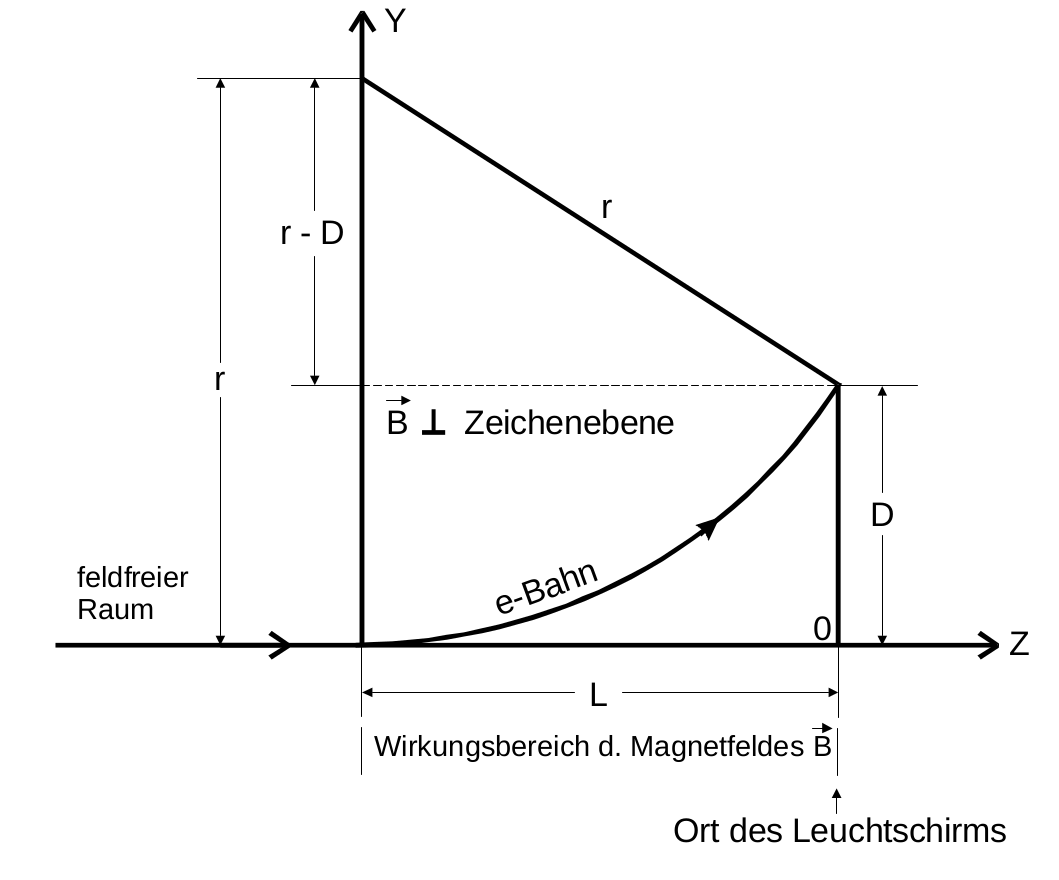
\includegraphics[width=0.8\textwidth]{Messdaten/ablenkungbfeld.png}
  \caption{Skizze der Elektronenbahn zur Bestimmung der Verschiebung $D$ am Leuchtschirm.}
  \label{fig:D}
\end{figure}
Wie aus Abbildung \ref{fig:D} ersichtlich, verursacht das Magnetfeld $\vec{B}$ eine Ablenkung um $D$ von der ursprünglichen Bahn des Elektron.
Die Größe $D$ kann am Schirm der Kathodenstrahlröhre gemessen werden.
Für den Bahnradius $r$ ergibt sich
\begin{equation}
  \label{eqn:dreii}
	r=\frac{L^2+D^2}{2D} \mathrm{.}
\end{equation}
Ein Gleichsetzen der Gleichungen \eqref{eqn:Radius} und \eqref{eqn:dreii} eliminiert den Bahnradius $r$. Unter Verwendung von Gleichung \eqref{eqn:vnull} ergibt sich
\begin{equation}
  \label{eqn:bfeld1}
  \frac{D}{L^2+D^2}=\frac{1}{\sqrt{8U_\mathrm{B}}}\sqrt{\frac{\symup{e}_0}{\symup{m}_0}}B \text{.}
\end{equation}
Im vorliegenden Experiment wird zur Erzeugung eines homogenen Magnetfeldes ein Helmholtzspulenpaar verwendet.
Die Flussdichte $B$ ist gegeben durch:
\begin{equation}
  B=\mu_0\frac{8}{\sqrt{125}}\frac{N\cdot I}{R} \text{.}
\end{equation}
Hierbei ist $N$ die Windungszahl und $I$ der Spulenstrom.
